\chapter{Ionen en ionenoplossingen}\label{ch:g9:ions}

Op een bank in de gymzaal staan twee heldere drankjes: een fles
sportdrank, verkocht om zijn ``elektrolyten'', en een glas suikerwater.
In een laboratorium worden twee metalen plaatjes, verbonden met een
batterij en een lampje, om de beurt in elk drankje gedompeld. In de
sportdrank gaat het lampje branden; in het suikerwater blijft het donker.
Iets in de eerste vloeistof draagt elektrische lading, en de suiker niet.
Dat iets zijn \omterm{def:g9:ions:ion}{ionen}.

\begin{recall}
Een \omterm{def:g7:atoms-and-molecules:atom}{atoom} heeft een kern met $Z$ \omterm{def:g9:inside-the-atom:proton}{protonen}, elk met lading $+e$, en $Z$
\omterm{def:g9:inside-the-atom:nucleus}{elektronen} eromheen, elk met lading $-e$: het \omterm{def:g7:atoms-and-molecules:atom}{atoom} is neutraal
(\cref{ch:g9:inside-the-atom}). Een stof die in water opgelost is, geeft
een \omterm{def:g6:solutions-and-solubility:solute}{waterige oplossing} (\cref{ch:g6:solutions-and-solubility}). Een
\omterm{def:g7:identifying-substances:characteristic-test}{aantoningsreactie} toont een stof aan door een zichtbaar resultaat
(\cref{ch:g7:identifying-substances}).
\end{recall}

\begin{omfigure}
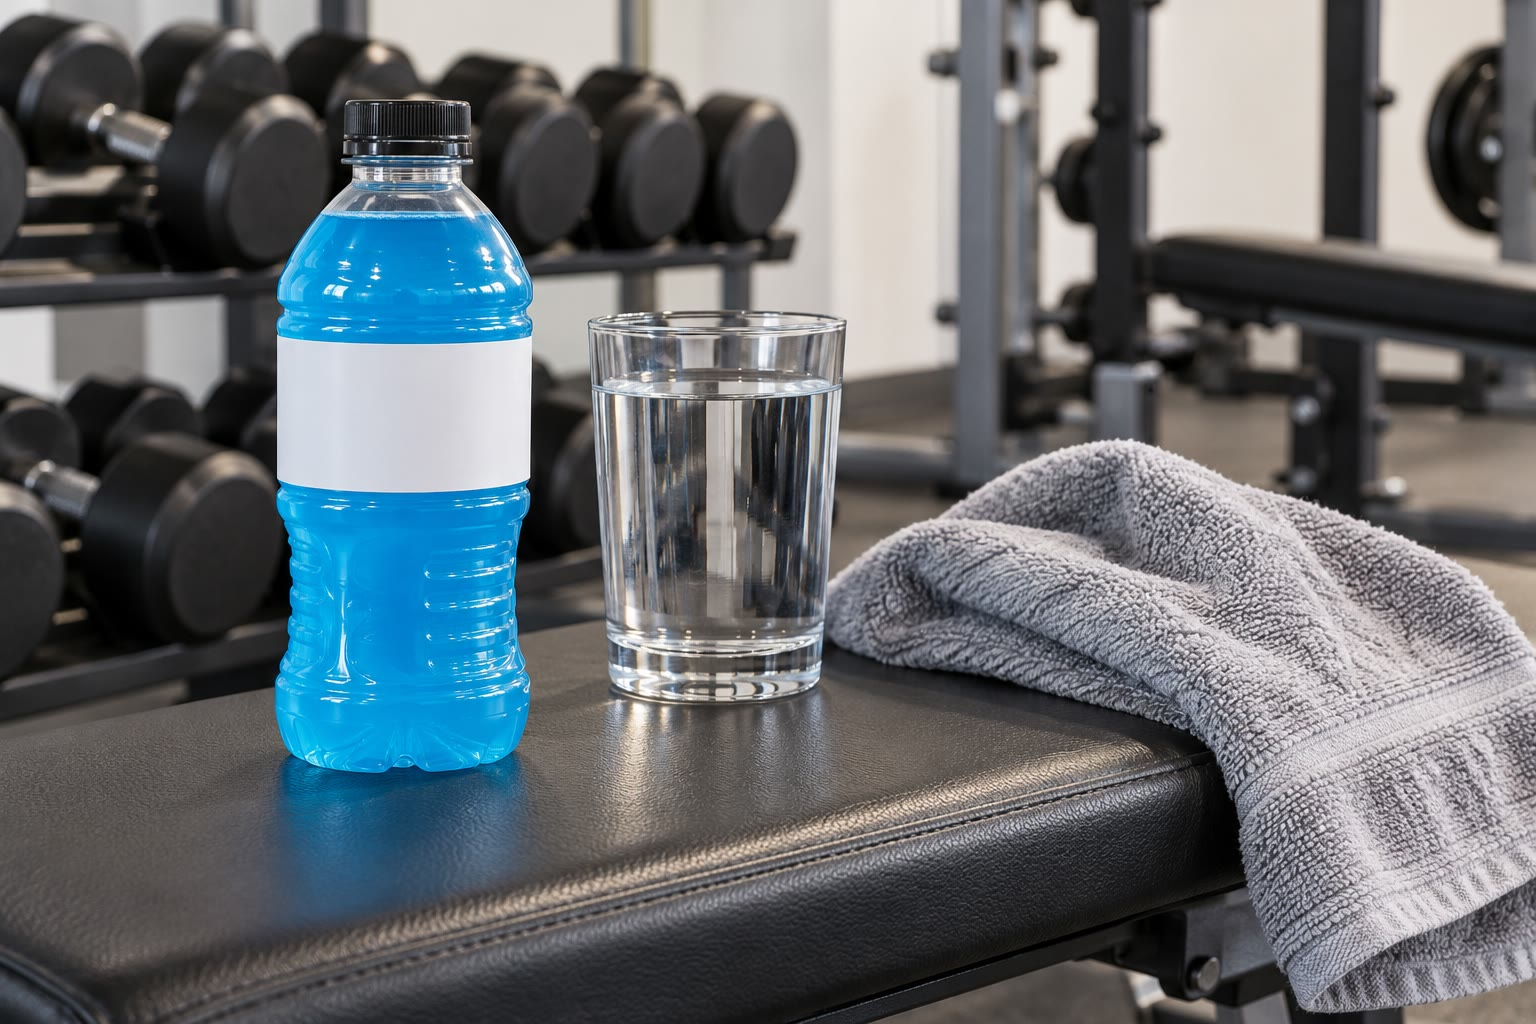
\includegraphics[width=0.5\linewidth]{images/book1/ai/g9-sports-drink.jpg}

{\small Een sportdrank en een glas water: in de drank zitten opgeloste
\omterm{def:g9:ions:ion}{ionen}.}
\end{omfigure}

\section{Atomen die elektronen opnemen of afstaan}

\begin{definition}[Ion, kation, anion]\label{def:g9:ions:ion}
Een \emph{ion}\index{ion} is een \omterm{def:g7:atoms-and-molecules:atom}{atoom}, of een groep \omterm{def:g7:atoms-and-molecules:atom}{atomen}, dat een of
meer \omterm{def:g9:inside-the-atom:nucleus}{elektronen} heeft afgestaan of opgenomen, en daardoor een elektrische
lading draagt. Een ion met een positieve lading, dat \omterm{def:g9:inside-the-atom:nucleus}{elektronen} heeft
afgestaan, is een \emph{kation}\index{kation}; een ion met een negatieve
lading, dat \omterm{def:g9:inside-the-atom:nucleus}{elektronen} heeft opgenomen, is een
\emph{anion}\index{anion}. De lading schrijf je rechtsboven de formule:
\ce{Na+}, \ce{Cu^{2+}}, \ce{Cl-}.
\end{definition}

\begin{example}[Natrium en chloor]\label{ex:g9:ions:na-cl}
Een natriumatoom, 11 \omterm{def:g9:inside-the-atom:proton}{protonen} en 11 \omterm{def:g9:inside-the-atom:nucleus}{elektronen}, staat één \omterm{def:g9:inside-the-atom:nucleus}{elektron} af:
het wordt het natriumion \ce{Na+}, 11 \omterm{def:g9:inside-the-atom:proton}{protonen} en 10 \omterm{def:g9:inside-the-atom:nucleus}{elektronen}, lading
$+1$:
\[
  \ce{Na -> Na+ + e-}.
\]
Een chlooratoom, 17 \omterm{def:g9:inside-the-atom:proton}{protonen} en 17 \omterm{def:g9:inside-the-atom:nucleus}{elektronen}, neemt één \omterm{def:g9:inside-the-atom:nucleus}{elektron} op:
het wordt het \omterm{def:g9:ions:ion}{chloride-ion} \ce{Cl-}, 17 \omterm{def:g9:inside-the-atom:proton}{protonen} en 18 \omterm{def:g9:inside-the-atom:nucleus}{elektronen}:
\[
  \ce{Cl + e- -> Cl-}.
\]
\end{example}

\begin{omfigure}
\begin{tikzpicture}[font=\small]
  \foreach \x/\name/\p/\e/\ch/\col in {0/{natrium\-atoom}/11/11/0/omDef,
      3.7/{natriumion \ce{Na+}}/11/10/+1/omProp,
      8.0/{chloor\-atoom}/17/17/0/omDef, 11.7/{chloride-ion \ce{Cl-}}/17/18/$-1$/omProp} {
    \node[draw=\col, fill=\col!6, rounded corners=2pt, align=center, text width=2.4cm]
      at (\x,0) {\textbf{\name}\\ \p\ protonen\\ \e\ elektronen\\ lading \ch};
  }
  \draw[->, thick, omProp] (1.45,0) -- (2.25,0) node[midway, above, text=black,
    font=\footnotesize, align=center] {geeft\\ 1 \ce{e-}};
  \draw[->, thick, omProp] (9.45,0) -- (10.25,0) node[midway, above, text=black,
    font=\footnotesize, align=center] {krijgt\\ 1 \ce{e-}};
\end{tikzpicture}

{\small Een natriumatoom wordt een natriumion door een \omterm{def:g9:inside-the-atom:nucleus}{elektron} af te
staan; een chlooratoom wordt een \omterm{def:g9:ions:ion}{chloride-ion} door er een op te nemen. De
\omterm{def:g9:inside-the-atom:proton}{protonen} veranderen niet.}
\end{omfigure}

\begin{proposition}[Enkele veelvoorkomende ionen]\label{prop:g9:ions:common}
Eenatomige \omterm{def:g9:ions:ion}{ionen} bestaan uit één \omterm{def:g7:atoms-and-molecules:atom}{atoom}; samengestelde \omterm{def:g9:ions:ion}{ionen} uit een groep
\omterm{def:g7:atoms-and-molecules:atom}{atomen} die bij elkaar blijft:
\begin{center}
\small
\begin{tabular}{llll}
\hline
\omterm{def:g9:ions:ion}{kationen} & & \omterm{def:g9:ions:ion}{anionen} & \\
\hline
natrium & \ce{Na+} & chloride & \ce{Cl-} \\
kalium & \ce{K+} & hydroxide & \ce{OH-} \\
calcium & \ce{Ca^{2+}} & nitraat & \ce{NO3-} \\
magnesium & \ce{Mg^{2+}} & carbonaat & \ce{CO3^{2-}} \\
koper(II) & \ce{Cu^{2+}} & sulfaat & \ce{SO4^{2-}} \\
ijzer(II), ijzer(III) & \ce{Fe^{2+}}, \ce{Fe^{3+}} & & \\
zink & \ce{Zn^{2+}} & & \\
aluminium & \ce{Al^{3+}} & & \\
ammonium & \ce{NH4+} & & \\
\hline
\end{tabular}
\end{center}
\end{proposition}

\section{Ionverbindingen en hun formules}

\begin{definition}[Ionverbinding]\label{def:g9:ions:ionic-compound}
Een \emph{ionverbinding}\index{ionverbinding} bestaat uit \omterm{def:g9:ions:ion}{kationen} en
\omterm{def:g9:ions:ion}{anionen} in zulke aantallen dat het geheel geen lading draagt. De formule
geeft de verhouding van de \omterm{def:g9:ions:ion}{ionen}, zonder hun ladingen: \ce{NaCl} voor
natriumchloride, één \ce{Na+} op elk \ce{Cl-}; \ce{CaCl2} voor
calciumchloride, twee \ce{Cl-} op elk \ce{Ca^{2+}}.
\end{definition}

\begin{method}[De formule van een ionverbinding opschrijven]\label{met:g9:ions:formula}
\begin{enumerate}
  \item Schrijf de twee \omterm{def:g9:ions:ion}{ionen} op met hun lading, het \omterm{def:g9:ions:ion}{kation} eerst.
  \item Zoek van elk het kleinste aantal waarbij de totale lading nul
        wordt.
  \item Schrijf die aantallen als \omterm{def:g7:atoms-and-molecules:formula}{index}; een samengesteld \omterm{def:g9:ions:ion}{ion} dat een
        \omterm{def:g7:atoms-and-molecules:formula}{index} nodig heeft, komt tussen haakjes.
\end{enumerate}
Aluminiumoxide: \ce{Al^{3+}} en \ce{O^{2-}}; $2 \times (+3) + 3 \times
(-2) = 0$, dus \ce{Al2O3}. IJzer(III)hydroxide: \ce{Fe^{3+}} en drie
\ce{OH-}: \ce{Fe(OH)3}.
\end{method}

\begin{proposition}[Een ionaire vaste stof is een stapeling van ionen]\label{prop:g9:ions:solid}
In een zoutkristal wisselen natriumionen en \omterm{def:g9:ions:ion}{chloride-ionen} elkaar af in
een regelmatige driedimensionale stapeling, elk \omterm{def:g9:ions:ion}{ion} omringd door \omterm{def:g9:ions:ion}{ionen}
met de tegengestelde lading, die het op zijn plaats houden. Een korrel
keukenzout bevat er miljarden miljarden; zijn kubusvorm weerspiegelt de
kubische stapeling.
\end{proposition}

\begin{omfigure}
\begin{minipage}[b]{0.5\linewidth}\centering
\begin{tikzpicture}[font=\small]
  \foreach \i in {0,...,5} \foreach \j in {0,...,4} {
    \pgfmathtruncatemacro\pp{mod(\i+\j,2)}
    \ifnum\pp=0 \node[aNa, minimum size=5mm] at (0.62*\i,0.62*\j) {};
    \else \node[aCl, minimum size=7.4mm] at (0.62*\i,0.62*\j) {};\fi
  }
\end{tikzpicture}

{\small Eén laag van een zoutkristal: natriumionen (paars, kleiner) en
\omterm{def:g9:ions:ion}{chloride-ionen} (groen) wisselen elkaar af.}
\end{minipage}\hfill
\begin{minipage}[b]{0.3\linewidth}\centering
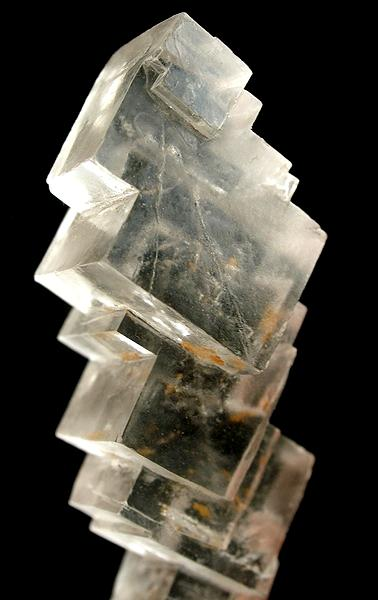
\includegraphics[height=4.6cm]{images/book1/halite.jpg}

{\small Haliet, natuurlijk steenzout. Foto: Robert M.~Lavinsky,
CC BY-SA 3.0.}
\end{minipage}
\end{omfigure}

\section{Ionenoplossingen geleiden}

\begin{notation}[De toestandsaanduiding (aq)]\label{not:g9:ions:aq}
Een \omterm{def:g9:ions:ion}{ion} of een \omterm{def:g7:atoms-and-molecules:molecule}{molecuul} dat in water opgelost is, krijgt (aq), van
het Latijnse aqua, water: \ce{Na+(aq)}, \ce{Cl-(aq)}.
\end{notation}

\begin{proposition}[Ionenoplossingen geleiden elektrische stroom]\label{prop:g9:ions:conduct}
Als een \omterm{def:g9:ions:ionic-compound}{ionverbinding} in water \omterm{def:g2:mixing-and-dissolving:dissolve}{oplost}, raken de \omterm{def:g9:ions:ion}{ionen} los van elkaar en
bewegen ze vrij door de oplossing: zout water bevat \ce{Na+(aq)} en
\ce{Cl-(aq)}. Bewegende \omterm{def:g9:ions:ion}{ionen} dragen elektrische lading, dus een
ionenoplossing geleidt elektrische stroom. Een suikeroplossing, waarvan
de \omterm{def:g7:atoms-and-molecules:molecule}{moleculen} geen lading dragen, geleidt niet; heel zuiver water ook
niet.
\end{proposition}

\begin{inthelab}[Welke vloeistoffen geleiden?]
De docent verbindt twee metalen plaatjes, een batterij met een lage
spanning en een lampje tot een stroomkring; de plaatjes worden om de
beurt gedompeld in gedestilleerd water, suikerwater, zout water en een
kopersulfaatoplossing, en tussendoor afgespoeld. Het lampje brandt alleen
bij de twee ionenoplossingen.
\end{inthelab}

\begin{omfigure}
\begin{tikzpicture}[font=\small, scale=1.1]
  \foreach \xs/\lit/\lab in {0/1/{zout water: het lampje brandt}, 5.2/0/{suikerwater: het blijft donker}} {
    \begin{scope}[xshift=\xs cm]
      \pic[transform shape] at (2,0) {beaker={0.7}{omWater!80}};
      \fill[black!45] (1.6,0.25) rectangle (1.7,2.6);
      \fill[black!45] (2.3,0.25) rectangle (2.4,2.6);
      \ifnum\lit=1 \fill[yellow!70, opacity=0.8] (3.4,3.0) circle (0.42);\fi
      \draw (1.65,2.6) -- (1.65,3.6) to[battery1] (3.4,3.6) -- (3.4,3.4)
        to[lamp] (3.4,2.6) -- (2.35,2.6);
      \node[anchor=north, align=center] at (2,-0.15) {\lab};
    \end{scope}
  }
\end{tikzpicture}

{\small De geleidbaarheidstest: met zout water dragen \omterm{def:g9:ions:ion}{ionen} de stroom en
brandt het lampje; suikerwater bevat geen \omterm{def:g9:ions:ion}{ionen} en het lampje blijft
donker.}
\end{omfigure}

\section{Neerslagreacties om ionen aan te tonen}

\begin{definition}[Neerslag]\label{def:g9:ions:precipitate}
Als je twee oplossingen \omterm{def:g2:mixing-and-dissolving:mix}{mengt}, kunnen een \omterm{def:g9:ions:ion}{kation} van de ene en een \omterm{def:g9:ions:ion}{anion}
van de andere een \omterm{def:g9:ions:ionic-compound}{ionverbinding} vormen die niet \omterm{def:g2:mixing-and-dissolving:dissolve}{oplost}. Die verschijnt
als een fijne vaste stof die de vloeistof troebel maakt en bezinkt: een
\emph{neerslag}\index{neerslag}. De reactie is een
\emph{neerslagreactie}\index{neerslagreactie}.
\end{definition}

\begin{proposition}[Aantoningsreacties voor veelvoorkomende ionen]\label{prop:g9:ions:tests}
Een paar druppels van een reagensoplossing tonen een \omterm{def:g9:ions:ion}{ion} aan door de
kleur van de \omterm{def:g9:ions:precipitate}{neerslag} die het vormt:
\begin{center}
\small
\begin{tabular}{llll}
\hline
gezocht \omterm{def:g9:ions:ion}{ion} & \omterm{def:g7:identifying-substances:characteristic-test}{reagens} & \omterm{def:g9:ions:precipitate}{neerslag} & kleur \\
\hline
koper(II) \ce{Cu^{2+}} & natriumhydroxide & \ce{Cu(OH)2} & blauw \\
ijzer(II) \ce{Fe^{2+}} & natriumhydroxide & \ce{Fe(OH)2} & groen \\
ijzer(III) \ce{Fe^{3+}} & natriumhydroxide & \ce{Fe(OH)3} & oranjebruin \\
zink \ce{Zn^{2+}} & natriumhydroxide & \ce{Zn(OH)2} & wit \\
aluminium \ce{Al^{3+}} & natriumhydroxide & \ce{Al(OH)3} & wit \\
chloride \ce{Cl-} & zilvernitraat & \ce{AgCl} & wit, kleurt donker in licht \\
\hline
\end{tabular}
\end{center}
\end{proposition}

\begin{example}[Een neerslagreactie opschrijven]\label{ex:g9:ions:equation}
Je schrijft alleen de \omterm{def:g9:ions:ion}{ionen} op die de vaste stof vormen; de andere
blijven opgelost en doen niet mee:
\[
  \ce{Cu^{2+}(aq) + 2OH-(aq) -> Cu(OH)2(s)}, \qquad
  \ce{Ag+(aq) + Cl-(aq) -> AgCl(s)}.
\]
\end{example}

\begin{omfigure}
\begin{tikzpicture}[font=\small, scale=0.95]
  \foreach \k/\pc/\lab in {0/blue!60/{\ce{Cu^{2+}}: blauw}, 1/green!45!black!70/{\ce{Fe^{2+}}: groen},
      2/orange!70!brown/{\ce{Fe^{3+}}: oranje-\\bruin}, 3/white!85!black/{\ce{Zn^{2+}}: wit},
      4/white!85!black/{\ce{Al^{3+}}: wit}, 5/white!80!black/{\ce{Cl-}: wit}} {
    \pic[transform shape] at (\k*2.3,0) {testtube={0.5}{omWater!60}};
    \pic[transform shape] at (\k*2.3,0) {testtube={0.14}{\pc}};
    \node[anchor=north, align=center, font=\footnotesize, text width=2cm] at (\k*2.3,-0.15) {\lab};
  }
\end{tikzpicture}

{\small \omterm{def:g9:ions:precipitate}{Neerslagen} gevormd met natriumhydroxide (eerste vijf buizen) en
met zilvernitraat (laatste buis).}
\end{omfigure}

\begin{safety}{\ghs[0.82cm]{GHS05}\ghs[0.82cm]{GHS07}}
% ledger: ghs:NaOH, ghs:AgNO3
Natriumhydroxide: veroorzaakt ernstige brandwonden en oogletsel, en kan
bijtend zijn voor metalen (GHS05); verdund irriterend voor huid en ogen
(GHS07). Zilvernitraat, het \omterm{def:g7:identifying-substances:characteristic-test}{reagens} op chloride, is oxiderend, bijtend
en zeer giftig voor in het water levende organismen. Veiligheidsbril,
handschoenen; de docent geeft de \omterm{def:g7:identifying-substances:characteristic-test}{reagentia} druppelsgewijs uit.
\end{safety}

\begin{method}[Een ion aantonen]\label{met:g9:ions:test}
\begin{enumerate}
  \item Giet een beetje van de te testen oplossing in een reageerbuis.
  \item Voeg het \omterm{def:g7:identifying-substances:characteristic-test}{reagens} druppel voor druppel toe.
  \item Noteer de kleur van een eventuele \omterm{def:g9:ions:precipitate}{neerslag} en vergelijk met de
        tabel.
  \item Trek je conclusie, en onthoud dat een test een \omterm{def:g9:ions:ion}{ion} aantoont,
        geen verbinding: een oplossing van ijzer(III)chloride geeft
        zowel de test op \ce{Fe^{3+}} als de test op \ce{Cl-}.
\end{enumerate}
\end{method}

\section{Oefeningen}

\begin{exercise}[$\star$]\label{exo:g9:ions:1}
Wat is een \omterm{def:g9:ions:ion}{ion}? Wat is het verschil tussen een \omterm{def:g9:ions:ion}{kation} en een \omterm{def:g9:ions:ion}{anion}?
\end{exercise}

\begin{exercise}[$\star$]\label{exo:g9:ions:2}
Een magnesiumatoom (12 \omterm{def:g9:inside-the-atom:proton}{protonen}) staat twee \omterm{def:g9:inside-the-atom:nucleus}{elektronen} af. Schrijf de
formule op van het \omterm{def:g9:ions:ion}{ion} dat ontstaat, en geef zijn aantal \omterm{def:g9:inside-the-atom:proton}{protonen} en
\omterm{def:g9:inside-the-atom:nucleus}{elektronen}.
\end{exercise}

\begin{exercise}[$\star$]\label{exo:g9:ions:3}
Schrijf de formules op van kaliumchloride, magnesiumchloride en
calciumoxide (\omterm{def:g9:ions:ion}{oxide-ion}: \ce{O^{2-}}).
\end{exercise}

\begin{exercise}[$\star$]\label{exo:g9:ions:4}
Waarom geleidt zout water elektrische stroom en suikerwater niet?
\end{exercise}

\begin{exercise}[$\star\star$]\label{exo:g9:ions:5}
Schrijf de formules op van koper(II)sulfaat, aluminiumchloride en
natriumcarbonaat.
\end{exercise}

\begin{exercise}[$\star\star$]\label{exo:g9:ions:6}
Natriumhydroxide geeft met een oplossing een oranjebruine \omterm{def:g9:ions:precipitate}{neerslag}.
Welk \omterm{def:g9:ions:ion}{ion} bevat de oplossing? Schrijf de vergelijking van de
\omterm{def:g9:ions:precipitate}{neerslagreactie} op.
\end{exercise}

\begin{exercise}[$\star\star$]\label{exo:g9:ions:7}
Hoeveel \omterm{def:g9:inside-the-atom:nucleus}{elektronen} draagt het sulfaation \ce{SO4^{2-}} meer dan het
\omterm{def:g9:inside-the-atom:proton}{protonen} heeft? En het nitraation \ce{NO3-}?
\end{exercise}

\begin{exercise}[$\star\star$]\label{exo:g9:ions:8}
Een oplossing geeft een witte \omterm{def:g9:ions:precipitate}{neerslag} met zilvernitraat en een blauwe
met natriumhydroxide. Geef de naam van de opgeloste \omterm{def:g9:ions:ionic-compound}{ionverbinding} en
schrijf haar formule op.
\end{exercise}

\begin{exercise}[$\star\star$]\label{exo:g9:ions:9}
Kijk naar de figuur van de laag van het zoutkristal. Hoeveel buren met
een tegengestelde lading heeft een \omterm{def:g9:ions:ion}{ion} midden in de laag binnen die
laag?
\end{exercise}

\begin{exercise}[$\star\star$]\label{exo:g9:ions:10}
Schrijf de vergelijking op van de \omterm{def:g9:ions:precipitate}{neerslagreactie} van ijzer(II)hydroxide
uit \ce{Fe^{2+}}- en \ce{OH-}-ionen.
\end{exercise}

\begin{exercise}[$\star\star\star$]\label{exo:g9:ions:11}
Een wit poeder kan zinkchloride of natriumchloride zijn. Opgelost in
water geeft het een witte \omterm{def:g9:ions:precipitate}{neerslag} met natriumhydroxide. Welke stof is
het? Schrijf de vergelijking op.
\end{exercise}

\begin{exercise}[$\star\star\star$]\label{exo:g9:ions:12}
Hoeveel \omterm{def:g9:ions:ion}{chloride-ionen} zijn er in een kristal calciumchloride op 1000
calciumionen? Controleer dat het kristal neutraal is.
\end{exercise}

\section{Probleem: De roestige put}

\begin{problem}[{Weekendprobleem --- oranje vlekken in de gootsteen van
een boerderij, twee tests, en het aantal ijzerionen in een liter
putwater}]
\label{pb:g9:ions:1}
Het water uit de put van een boerderij laat oranje vlekken achter in de
gootsteen. Een laboratorium krijgt een monster. Vers opgepompt is het
water helder; met natriumhydroxide geeft het een groene \omterm{def:g9:ions:precipitate}{neerslag}, die
binnen een uur aan het oppervlak, waar hij met de \omterm{def:g4:air-a-mixture-of-gases:air}{lucht} in aanraking
komt, oranjebruin wordt. Het laboratorium meet \qty{0.30}{mg} ijzer, in
de vorm van ijzerionen, per liter. Neem voor de massa van een \omterm{def:g9:inside-the-atom:proton}{nucleon}
\qty{1.67e-27}{kg}, en 56 \omterm{def:g9:inside-the-atom:proton}{nucleonen} voor een ijzeratoom.

\medskip
\noindent\textbf{Deel I --- De tests.}
\begin{enumerate}
  \item Welk \omterm{def:g9:ions:ion}{ion} toont de groene \omterm{def:g9:ions:precipitate}{neerslag} aan? Geef de formule van de
        \omterm{def:g9:ions:precipitate}{neerslag}.
  \item Welk \omterm{def:g9:ions:ion}{ion} toont de oranjebruine \omterm{def:g9:ions:precipitate}{neerslag} aan? Geef de formule.
  \item Een ijzer(II)\omterm{def:g9:ions:ion}{ion} en een ijzer(III)\omterm{def:g9:ions:ion}{ion} verschillen één \omterm{def:g9:inside-the-atom:nucleus}{elektron}.
        Welk van de twee heeft meer \omterm{def:g9:inside-the-atom:nucleus}{elektronen}? Hoeveel \omterm{def:g9:inside-the-atom:nucleus}{elektronen} heeft
        elk (ijzer: $Z = 26$)?
  \item Schrijf de vergelijking op van de \omterm{def:g9:ions:precipitate}{neerslagreactie} van
        ijzer(III)hydroxide.
\end{enumerate}

\medskip
\noindent\textbf{Deel II --- De vlekken.}
\begin{enumerate}[resume]
  \item In de gootsteen wordt het heldere water langzaam troebel en
        oranje. Welk \omterm{def:g9:ions:ion}{ion} bevat het water als het uit de put komt, en
        welk bevat het uiteindelijk?
  \item Schrijf de formule op van de \omterm{def:g9:ions:ionic-compound}{ionverbinding} die ijzer(III)\omterm{def:g9:ions:ion}{ionen} en
        \omterm{def:g9:ions:ion}{hydroxide-ionen} vormen, en controleer dat ze neutraal is.
  \item Kun je het ijzer uit het water halen door het water te
        \omterm{def:g3:separating-mixtures:filter}{filtreren} zodra het uit de put komt? En nadat het oranje is
        geworden? Leg uit.
  \item Is water dat ijzerionen bevat een \omterm{def:g6:pure-substances-and-mixtures:pure-substance}{zuivere stof}? Een \omterm{def:g6:pure-substances-and-mixtures:homogeneous}{homogeen
        mengsel}?
\end{enumerate}

\medskip
\noindent\textbf{Deel III --- De \omterm{def:g9:ions:ion}{ionen} tellen.}
\begin{enumerate}[resume]
  \item Bereken de massa van een ijzeratoom, in kilogram.
  \item Reken \qty{0.30}{mg} om naar kilogram.
  \item Waarom mag je de massa van een ijzerion gelijk nemen aan die van
        een ijzeratoom?
  \item Bereken het aantal ijzerionen in een liter putwater.
\end{enumerate}
\end{problem}
